\chapter{Locality and Caches}
\label{chap:locality}

For modern computers, computation is a rather cheap operation in terms
of time and energy consumption.  In fact, it is far more
energy-consuming and slow to \emph{move} data than to perform
computation.  As we discussed in \cref{chap:bytes}, program data is
usually stored in memory and must be moved into CPU registers before
it can be worked on.  Particularly large quantities of data might not
even fit in memory, but is stored in local or remote files.  The
details can differ, but in all cases the situation is the same: data
must be moved from \emph{over there} to \emph{here} before it can be
used.

This phenomenon that computation is faster than memory, is often
called the \emph{memory wall}, and the gap is still widening.  While
faster processors keep getting designed, memory technology is not
keeping up, and therefore we have increasing difficulty supplying our
processors with data.

Since data movement is slow and costly compared to computation, a
programmer who wants to write high-performance code must be diligent
in doing as little of it as possible.  This chapter describes the
properties of software and hardware that one must exploit to
accomplish this.

While we will continue to use C for concrete programming examples, the
principles here are truly universal, and inescapable whenever we write
code for modern computers.  Fortunately, we will see that optimising
code to minimise data movement usually doesn't require us to write
particularly ugly or complicated code - it is mostly about choosing
the right data structures and traversing them in a sensible manner.

\section{Locality of Reference}

Empirically, programs tend to access data located nearby data that was
accessed recently.  We call this phenomenon the \emph{principle of
  localty}.

\begin{definition}[Principle of locality]
  Programs tend to access data located near that which was accessed
  recently.
\end{definition}

To keep things simple, this chapters is concerned only with data
stored in memory, and we will decide if two pieces of data are
``close'' to each other based on the numerical value of their
addresses.  For example, the byte at address $100$ is considered
adjacent to the bytes at addresses $99$ and $101$.  However, some
notion of locality is present in any kind of storage technology.
Informally, we say that a program ``exhibits good locality'' when it
adheres to the principle of locality.

The principle of locality is what ultimately helps us break through
the memory wall.  It is a virtuous cycle: we build computers that take
run programs with good locality more quickly, which makes programs try
to improve the locality in their programs.

We distinguish between two kinds of locality.

\begin{definition}[Temporal locality]
  Accessing data that was accessed recently.
\end{definition}

\begin{definition}[Spatial locality]
  Accesing data close to data that was accessed recently.
\end{definition}

While it is possible to run a program, record the exact memory
operations performed, and then quantiatively describe how much
locality they exhibit, this is often somewhat impractical.  Instead, a
good programmer should develop the ability to quickly eyeball simple
programs and qualitiatively estimate their locality.

\subsection{Qualitative Estimates of Locality}

\begin{figure}
\begin{lstlisting}[
caption={C code that sums an array.},
label={lst:locality-example},
language=C,
frame=single]
double sum = 0;
for (int i = 0; i < n; i++) {
  sum += a[i];
}
\end{lstlisting}
\end{figure}

Consider the program fragment shown in \cref{lst:locality-example}.
In terms of data accesses, it accesses the elements of the array
\texttt{a} serially, with a \emph{stride} of $1$ between successive
accesses.  This is an example of \emph{spatial locality}: we do not
access the same data, but we do access data very close to what we
accessed in the recent past.  Further, we also repeatedly access the
variables \texttt{sum} and \texttt{i}. This is an example of
\emph{temporal locality}.

But program data is not the only thing that is stored in memory: the
program \emph{code} is as well, in the form of machine instructions.
Absent of control flow, instructions are read from memory and executed
in the order in which they appear---just like how lines in a C program
are executed from the top down.  This means they have \emph{spatial
  locality}.  However, we also have a loop in
\cref{lst:locality-example}, which means that the same instructions
are executed repeatedly.  This is \emph{temporal locality}.  Generally
speaking, program code almost always exhibits good locality, so we
tend to ignore it when analysing the locality of a program, and
instead focus only on the locality of data accesses.

Further, we focus only on memory accesses.  Because simple scalar
variables tend to be stored in registers by the C compiler, we look
only at how arrays are traversed.

\subsection{Analysing Array Iteration}

\begin{figure}
\begin{lstlisting}[
caption={Summing a matrix, iterating along the rows.},
label={lst:locality-sumrows},
language=C,
frame=single]
int sumrows(int A[M][N]) {
  int sum = 0;
  for (int i = 0; i < M; i++)
    for (int j = 0; j < N; j++)
      sum += A[i][j];
  return sum;
}
\end{lstlisting}
\end{figure}

Let us consider a more complicated example, seen in
\cref{lst:locality-sumrows}.  For concision we are use
multidimensional C arrays, rather than explicit index functions as in
\cref{chap:datalayout}.  This means that the array \texttt{A} is
stored in row-major order and that the access \texttt{A[i][j]} results
in an offset computation \texttt{i*N+j}.

Consider the memory accesses performed by the loop.  In the first
iteration, we have \texttt{i=0} and \texttt{j=0}, meaning that we
access memory at offset \texttt{0}.  In the next iteration we have
\texttt{i=0} and \texttt{j=1}, meaning we access offset
\texttt{1}\footnote{Strictly speaking, we are accessing
  \texttt{1*sizeof(int)}, meaning \texttt{4}, but since the first
  iteration accesses the four bytes stored at offsets \texttt{0-3},
  this is still considered adjacent.  We can ignore the element size
  for arrays of scalars, but it does have impact if we have arrays
  containing large compound data structures.}.  In every loop
iteration, we will access an array element adjacent to the one
accessed in the immediately preceding iteration---the stride is
$1$---and therefore this function exhibits good spatial locality with
respect to how it accesses \texttt{A}.

\begin{figure}
\begin{lstlisting}[
caption={Summing the rows of a matrix, iterating along the columns},
label={lst:locality-sumcols},
language=C,
frame=single]
int sumcols(int A[M][N]) {
  int sum = 0;
  for (int j = 0; j < N; j++)
    for (int i = 0; i < M; i++)
      sum += A[i][j];
  return sum;
}
\end{lstlisting}
\end{figure}

Now consider \cref{lst:locality-sumcols}.  By repeating the analysis
above, we see that the first array element we access is
\texttt{A[0][0]} and the next one is \texttt{A[1][0]}.  Since
\texttt{A} is stored in row-major order, this means we are iterating
with a stride of \texttt{N}.  Assuming \texttt{N} is large, this
function exhibits \emph{bad} locality with respect to \texttt{A}.

\section{Memory Hierarchies}

In an ideal world, memory would be cheap, fast, and plentiful.  In the
world we actually inhabit, we cannot get all three.  In fact,
fundamental physical principles mean memory capacity and memory
capacity are conflicting properties.  Roughly, the larger the capacity
of some storage technology, the longer it takes it to retrieve data.
However, by exploiting the principle of locality, we can construct a
\emph{memory hierarchy} of different storage technologies, starting
from the small and fast and ending in the large and slow.

\begin{definition}[Memory hierarchy]
  A separation of computer storage into levels based on their response
  time and capacity.
\end{definition}

The idea behind a memory hierarchy is that each level contains a
\emph{subset} of the data contained in the level below it.  Only the
level at the bottom contains \emph{all} data.  Each level of the
hierarchy acts as a \emph{cache} for the one below it.

\begin{definition}[Cache]
  A smaller and faster memory that stores a subset of the contents of
  a larger and slower memory.
\end{definition}


\begin{figure}
  \centering

  \begin{center}
    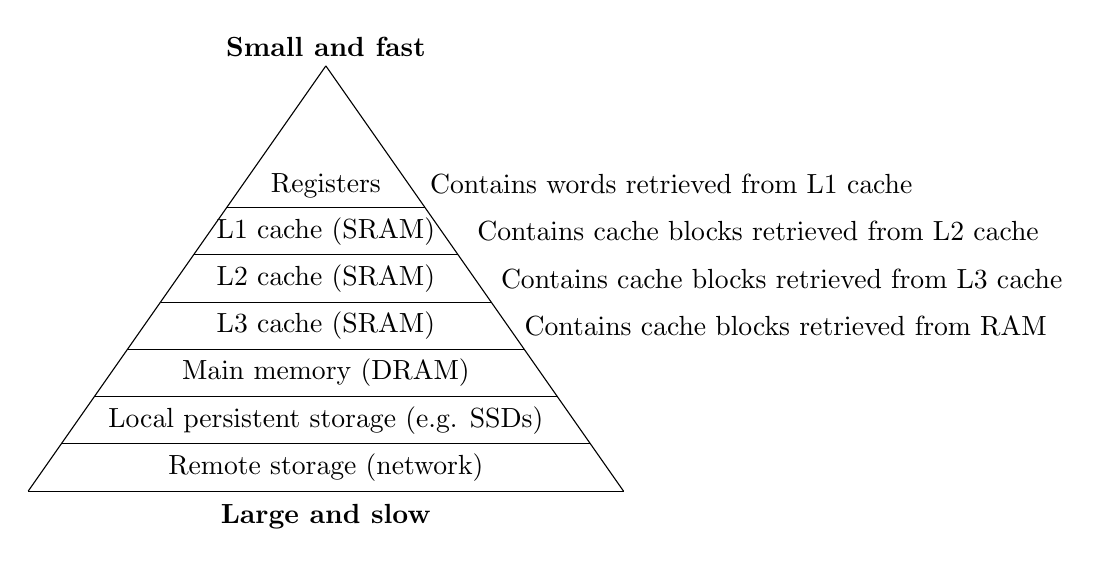
\begin{tikzpicture}[scale=0.6]
      \def \h {9};
      \def \f {.7};

      \foreach \y in  {0,1,2,3,4,5,6} {
        \def \w { \h*\f-\y*\f };
        \def \v { \y*\f-\h*\f };
        \draw (\v,\y) -- (\w,\y);
      }

      \draw (-\h*\f,0)  -- (0,\h);
      \draw (\h*\f,0)  -- (0,\h);

      \node at (0,0) [above] {Remote storage (network)};
      \node at (0,1) [above] {Local persistent storage (e.g. SSDs)};
      \node at (0,2) [above] {Main memory (DRAM)};
      \node at (0,3) [above] {L3 cache (SRAM)};
      \node[align=left] at (4,3.5) [right] {Contains cache blocks retrieved from RAM};
      \node at (0,4) [above] {L2 cache (SRAM)};
      \node[align=left] at (3.5,4.5) [right] {Contains cache blocks retrieved from L3 cache};
      \node at (0,5) [above] {L1 cache (SRAM)};
      \node[align=left] at (3,5.5) [right] {Contains cache blocks retrieved from L2 cache};
      \node at (0,6) [above] {Registers};
      \node at (2,6.5) [right] {Contains words retrieved from L1 cache};

      \node at (0,9) [above] {\textbf{Small and fast}};
      \node at (0,-1) [above] {\textbf{Large and slow}};
    \end{tikzpicture}
  \end{center}

  \caption{Example memory hierarchy for a modern computer.  The number
    of levels and the specifics of their operation depends on the
    computer in question.  Very tiny computers may have no caches at
    all, but only registers and main memory.  Some extremely small
    processors may have only registers---but these are unlikely to be
    useful for general-purpose computation.}
  \label{fig:memory-hierarchy}
\end{figure}

An example of a memory hierarchy for a computer is shown in
\cref{fig:memory-hierarchy}.  The exact levels of the memory hierarchy
depends on the machine.  Further, when using the memory hierarchy
model to describe the performance of a system, we often exclude levels
that are irrelevant---for example, registers are often ignored because
they are controlled by the compiler, and we might ignore anything
below main memory if we know that our data will fit.

In this chapter we will focus entirely how the contents of RAM is
cached.  Further, while real computers usually have multiple levels of
caching, we will for simplicity asumme only a single level above main
memory, and just call it \emph{the cache}.  So in total, we pretend we
have only two levels: the small and fast cache on top, and the large
and slow main memory below it.  In a full memory hierarchy, this
situation is simply replicated for each levelall the way down.

\subsection{Cache Operation}

The reason why caching works is due to the principle of locality: most
accesses will tend to be towards the top of the hierarchy.  When we
try to access an address that is already present in the cache, the
data is immediately returned to the program.

\begin{definition}[Cache hit]
  A memory operation to an address that is present in the cache.
\end{definition}

If we try to retrieve a piece of data that is not already in the
cache, the data is fetched from the next level of the hierarchy,
stored in the cache, and then returned to the program.

\begin{definition}[Cache miss]
  A memory operation to an address that is not present in the cache.
\end{definition}

In programs with good locality, most memory accesses will result in
cache hits.  For such programs, the memory hierarchy provides the
illusion of storage that is as large as the bottommost level of the
hierarchy, and as fast as the topmost one.

If caches merely contained \emph{exactly} the bytes that had been
retrieved previously, then only temporal locality would benefit.
Instead, we partition the addressable memory space into \emph{cache
  blocks}, each containing $B$ bytes.

\begin{definition}[Cache block]
  A $B$-byte chunk of memory, where $B$ is a power of two.
\end{definition}

Whenever we have a cache miss, the entire block containing the
requested address is copied into the cache.  This means that
subsequent accesses to addresses that fall within the same block will
result in cache hits.  This means that programs that exhibit good
spatial locality will have more cache hits.

On modern computers, $B=64$ is common.  It is important to be aware
that the organisation of memory into cache blocks does not affect
addressing: data is still byte-addressed, and programs are not
directly aware of $B$.  We merely say that the first $B$ bytes of
memory belong to the first cache block, the next $B$ bytes to the
second, and so on.  This means a memory address $x$ belongs to block
$x mod B$.  When $B$ is a power of 2 $B=2^{m}$, this can be computed
simply by dropping the $b$ least significant bits of $m$.  We will
return to this in \cref{sec:cache-organisation}.  Each level of the
memory hierarchy may use different cache block sizes, although they
are usually the same for the L1/L2/L3 caches.

Caching is effective when the data being actively actively by the
program within some bounded period of time fits within the cache.  We
call the size of this actively used data the \emph{working set}.

\begin{definition}[Working set]
  The amount of memory accessed by a program within a bounded period
  of time.
\end{definition}

\begin{definition}[Memory footprint]
  The total amount of memory allocated by a program.
\end{definition}

During the total runtime of a process, different working sets may be
in use, as the program switches between different subtasks.  Consider
a data analysis program sequentially processes a collection of files,
one at a time, by loading them into memory.  We would characterise the
working set of such a program as the size of a \emph{single} file
(perhaps the largest one), rather than summing the sizes of all files.
We also focus only on data that is being frequently accessed.  It is
fine for the total memory footprint of a program to exceed what can be
stored in the cache, as the excess is simply stored further down in
the memory hierarchy.  It is not unusual for programs to keep large
amounts of data in memory at the same time, while actively working on
only small parts at a time.  Indeed, this is exactly how to make best
use of the memory hierarchy.

\begin{definition}[Compulsory miss]
  A miss that occurs because the cache is empty.
\end{definition}

\begin{definition}[Capacity miss]
  A miss that occurs because the program working set exceeds the cache
  capacity.
\end{definition}

\section{Cache Organisation}
\label{sec:cache-organisation}

In this section we will look at how caches are organised in terms of
logical units.  Their physical representation may be different, but
this need not concern us.  What matters is how we can characterise the
structure of caches and how this affects the way we should program in
order to get optimal performance.  Beyond storing the actual cache
block data, caches must also maintain a variety of book-keeping
information so they can quickly determine whether a given address
corresponds to a block that is present.  We call a cache block
alongside this auxiliary information a \emph{cache line}.  when
describing the size of a cache, we count only the cache blocks, even
though the auxiliary information may take up a significant amount of
space.

\begin{definition}[Cache line]
  A structure that contains a cache block as well as metadata about
  the origin of the block.
\end{definition}

Be aware that this nomenclature is not universally used---many
programmers use the term \emph{cache line} interchangeably for both
what we call a cache block and a cache line.  For clarity, we will use
more precise nomenclature.

Specifically, a cache line contains three parts:

\begin{enumerate}
\item A cache block containing $B$ bytes.
\item A $t$-bit \emph{tag} indicating which part of memory is stored
  in the block.  The actual $t$ depends on the specific design of the
  cache.
\item A \emph{valid bit} indicating whether the cache line contents
  are sensible.
\end{enumerate}

The reason for the valid bit is that as a piece of hardware, a cache
line cannot be ``empty''.  There are always bits stored in the tag and
block fields, and they might accidentally correspond to a valid
address.  The valid bit is used to indicate whether the cache line
should be disregarded when checking whether the cache contains a block
corresponding to a given address.

At a high level, looking up an address $x$ in a cache then involves
computing the tag of the address as
\[
  x~\text{mod}~B
\]
and then searching for a cache line with a matching tag field.
However, for large caches, searching every single cache line would be
slow.  It is generally the case that the more choices you have, the
slower you are at making a choice.  Since the speed of cache lookups
is extremely critical for computer performance, this is not something
we want to make slower than absolutely necessary.

To solve this, we use \emph{set-associative caches}, where the lines
are split into $S$ \emph{sets}, with each set containing $L$ cache
lines, such that the total number of cache lines is $S\cdot{}L$.  The
bits of an address are then used to determine which set the block
corresponding to the address may be stored in.  The end result is that
we have only $L$ lines to search, rather than all lines in the cache.

\begin{definition}[$S$-way set associative cache]
  A cache with $S$ sets.
\end{definition}

When the number of sets and the block size are both powers of two
$S=2^{s}, B=2^{b}$, we can split a $w$-bit address into fields,
writing $x_{i}$ for bit $i$.

\[
  \underbrace{x_{w-1}\cdots{}x_{s+b+1}}_{\text{tag}}
  \underbrace{x_{b+s}\cdots{}x_{s}}_{\text{set index}}
  \underbrace{x_{b-1}\cdots{}x_{0}}_{\text{block offset}}
\]

\begin{example}[Fields for an 8-bit address scheme]
  Consider an $8$-bit address on a system with a block size of
  $B=2^{2}$ and $S=2^{3}$ sets, with.  Going from right to left, the
  first $b=2$ bits constitute the offset, the next $s=3$ bits the set
  index, and the remainder are the tag.
  \[
    \underbrace{x_{7}x_{6}x_{5}}_{\text{tag}}
    \underbrace{x_{4}x_{3}x_{2}}_{\text{tag}}
    \underbrace{x_{1}x_{0}}_{\text{offset}}
  \]
\end{example}

In a set-associative cache, a cache block is limited to being stored
in only a subset of all cache lines.  This means we risk having cache
misses even through the working set of the program is smaller than the
total size of the cache.  This is called a \emph{conflict miss}.

\begin{definition}[Conflict miss]
  A miss that occurs because too many blocks of the program working
  set are mapped to the same cache set.
\end{definition}

\begin{figure}
  \centering

  \begin{tikzpicture}
    \node (set4) at (-0.1,0.9) [draw,rectangle,anchor=south west,minimum width=7.7cm,minimum height=0.7cm] {};
    \draw (0,1) rectangle +(2,0.5) node (set40) {};
    \draw (2.5,1) rectangle +(2,0.5) node (set41) {};
    \node[align=center] at (5,1.25) {$\cdots$};
    \draw (5.5,1) rectangle +(2,0.5) node (set42) {};

    \node at (3.5,2.1) {$\vdots$};

    \node (set3) at (-0.1,2.4) [draw,rectangle,anchor=south west,minimum width=7.7cm,minimum height=0.7cm] {};
    \draw (0,2.5) rectangle +(2,0.5) node (set30) {};
    \draw (2.5,2.5) rectangle +(2,0.5) node (set31) {};
    \node[align=center] at (5,2.75) {$\cdots$};
    \draw (5.5,2.5) rectangle +(2,0.5) node (set32) {};

    \node (set2) at (-0.1,3.4) [draw,rectangle,anchor=south west,minimum width=7.7cm,minimum height=0.7cm] {};
    \draw (0,3.5) rectangle +(2,0.5) node (set20) {};
    \draw (2.5,3.5) rectangle +(2,0.5) node (set21) {};
    \node[align=center] at (5,3.75) {$\cdots$};
    \draw (5.5,3.5) rectangle +(2,0.5) node (set22) {};

    \node (set1) at (-0.1,4.4) [draw,rectangle,anchor=south west,minimum width=7.7cm,minimum height=0.7cm] {};
    \draw (0,4.5) rectangle +(2,0.5) node (set10) {};
    \draw (2.5,4.5) rectangle +(2,0.5) node (set11) {};
    \node[align=center] at (5,4.75) {$\cdots$};
    \draw (5.5,4.5) rectangle +(2,0.5) node (set12) {};

    \node (setlabel) at (9,5) {Set};
    \draw[->] (setlabel) -- (set1);

    \node (linelabel) at (9,4) {Line};
    \draw[->] (linelabel) -- (6.5,4.75);

    \draw [decorate,decoration={brace,amplitude=10pt,mirror}]
    (set1.north west) -- (set4.south west) node [black,midway,xshift=-1.3cm] {$S=2^{s}$ sets};

    \draw [decorate,decoration={brace,amplitude=10pt}]
    (set1.north west) -- (set1.north east) node [black,midway,yshift=0.8cm] {$L=2^{l}$ lines per set};

    \node[draw, minimum height=7mm] (validbit) {valid?};
    \node[draw, minimum height=7mm, right=2mm of validbit] (tag) {tag};
    \node[draw, minimum height=7mm, right=2mm of tag] (b0) {0};
    \node[draw, minimum height=7mm, right=0 of b0] (b1) {$1$};
    \node[draw, minimum height=7mm, right=0 of b1] (b2) {$2$};
    \node[draw, minimum height=7mm, right=0 of b2] (b3) {$\cdots$};
    \node[draw, minimum height=7mm, right=0 of b3] (b4) {$B-1$};

    \node[draw, fit=(validbit) (b4)] (cacheline) {};

    \draw [decorate,decoration={brace,amplitude=20pt,raise=10pt}]
    (b4.east) -- (b0.west) node [black,midway,yshift=-1.2cm] {$B=2^{b}$ bytes (cache block)};

    \draw[densely dotted] (cacheline.north west) -- (2.5,1);
    \draw[densely dotted] (cacheline.north east) -- (4.5,1);
  \end{tikzpicture}

  \caption{Structure of a set-associative cache with $S$ sets, $L$
    lines per set, and a $B$-byte block per line, where we assume all
    of these are powers of $2$.  The total size of this cache is
    $S \times L \times B$.}
  \label{fig:setassoc-cache}
\end{figure}

The general structure of a set-associative cache is shown in
\cref{fig:setassoc-cache}.  When designing a cache, the number of sets
must be carefully balanced: too large, and cache lookups take too
long.  Too small, and we end up with more conflict misses.  Balancing
this tradeoff is a delicate affair.  As of this writing, most CPU
caches are 8- or 16-way set associative.  Two special cases have
dedicated nomenclature.

\begin{definition}[Direct-mapped cache]
  A cache with $L=1$, meaning that there is only one possible location
  for a block in the cache.
\end{definition}

\begin{definition}[Fully associative cache]
  A cache with $S=1$, meaning that a block can be located anywhere in
  the cache.
\end{definition}

Direct-mapped and fully associative caches tend not to occur for CPU
caches, but they appear in lower parts of the memory hierarchy---the
latter typically when cache misses are ruinously expensive and so it
is worth significant overhead to avoid them.

\begin{figure}
  \centering

  \begin{tikzpicture}
    \node (set4) at (-0.1,0.9) [draw,rectangle,anchor=south west,minimum width=7.7cm,minimum height=0.7cm] {};
    \draw (0,1) rectangle +(2,0.5) node (set40) {};
    \draw (2.5,1) rectangle +(2,0.5) node (set41) {};
    \node[align=center] at (5,1.25) {$\cdots$};
    \draw (5.5,1) rectangle +(2,0.5) node (set42) {};

    \node at (3.5,2.1) {$\vdots$};

    \node (set3) at (-0.1,2.4) [draw,rectangle,anchor=south west,minimum width=7.7cm,minimum height=0.7cm] {};
    \draw (0,2.5) rectangle +(2,0.5) node (set30) {};
    \draw (2.5,2.5) rectangle +(2,0.5) node (set31) {};
    \node[align=center] at (5,2.75) {$\cdots$};
    \draw (5.5,2.5) rectangle +(2,0.5) node (set32) {};

    \node (set2) at (-0.1,3.4) [draw,rectangle,anchor=south west,minimum width=7.7cm,minimum height=0.7cm] {};
    \draw (0,3.5) rectangle +(2,0.5) node (set20) {};
    \draw (2.5,3.5) rectangle +(2,0.5) node (set21) {};
    \node[align=center] at (5,3.75) {$\cdots$};
    \draw (5.5,3.5) rectangle +(2,0.5) node (set22) {};

    \node (set1) at (-0.1,4.4) [draw,rectangle,anchor=south west,minimum width=7.7cm,minimum height=0.7cm] {};
    \draw (0,4.5) rectangle +(2,0.5) node (set10) {};
    \draw (2.5,4.5) rectangle +(2,0.5) node (set11) {};
    \node[align=center] at (5,4.75) {$\cdots$};
    \draw (5.5,4.5) rectangle +(2,0.5) node (set12) {};

    \draw [decorate,decoration={brace,amplitude=10pt,mirror}]
    (set1.north west) -- (set4.south west) node [black,midway,xshift=-1.3cm] {$S=2^{s}$ sets};

    \draw [decorate,decoration={brace,amplitude=10pt}]
    (set1.north west) -- (set1.north east) node [black,midway,yshift=0.8cm] {$L=2^{l}$ lines per set};

    \node at (10,5.7) {\textbf{Address components}};
    \node[draw, minimum height=7mm] (tagbits) at (9,5) {$t$ bits};
    \node[draw, minimum height=7mm, right=0mm of tagbits] (setbits) {$s$ bits};
    \node[draw, minimum height=7mm, right=0mm of setbits] (blockbits) {$b$ bits};
    \draw[decorate,decoration={brace,amplitude=10pt,mirror}]
    (tagbits.south west) -- (tagbits.south east) node [black,midway,yshift=-5mm,align=center,anchor=north] {tag};
    \draw[decorate,decoration={brace,amplitude=10pt,mirror}]
    (setbits.south west) -- (setbits.south east) node [black,midway,yshift=-5mm,align=center,anchor=north] {set\\ index};
    \draw[decorate,decoration={brace,amplitude=10pt,mirror}]
    (blockbits.south west) -- (blockbits.south east) node [black,midway,yshift=-5mm,anchor=north,align=center] {block\\offset};

    \draw[line width=1pt] let \p1 = (set4) in (10,3) -- (10,\y1) -- (set4.east);
    \draw[line width=1pt] (9,3.5) -- +(0,-2.8) -- +(-7.8,-2.8) -- +(-7.8,-2.5);
    \draw[line width=1pt] (3.2,0.7) -- +(0,0.3);
    \draw[line width=1pt] (6.2,0.7) -- +(0,0.3);
    \node[draw, minimum height=7mm] (validbit) {valid?};
    \node[draw, minimum height=7mm, right=2mm of validbit] (tag) {tag};
    \node[draw, minimum height=7mm, right=2mm of tag] (b0) {0};
    \node[draw, minimum height=7mm, right=0 of b0] (b1) {$1$};
    \node[draw, minimum height=7mm, right=0 of b1] (b2) {$2$};
    \node[draw, minimum height=7mm, right=0 of b2] (b3) {$\cdots$};
    \node[draw, minimum height=7mm, right=0 of b3] (b4) {$B-1$};
    \node[draw, fit=(validbit) (b4)] (cacheline) {};
    \draw[densely dotted] (cacheline.north west) -- (0,1);
    \draw[densely dotted] (cacheline.north east) -- (2,1);
    \draw[line width=1pt] (1.2,0.7) -- +(0,-0.3);
    \draw[line width=1pt] (11,3) -- +(0,-3.8) -- +(-8,-3.8) -- (b3.south west);
  \end{tikzpicture}

  \caption{Looking up an address in a set-associative cache with $S$
    sets and $L$ lines per set.  The set index determines which set to
    look at (in this case, the last one).  The set is then searched
    for a cache line with a tag matching the tag bits of the address.
    If a match is found (in this case, the first line), and the valid
    bit is set, the block offset of the address is used to determine
    which bytes to read from the block.}
  \label{fig:setassoc-cache-lookup}
\end{figure}

A diagram of how we perform a cache lookup based on an address is
shown in \cref{fig:setassoc-cache-lookup}.

\section{Cache Performance}

To characterise the cache behaviour of a program, we focus on the
\emph{miss rate}.
\begin{definition}[Miss rate]
  The fraction of memory references issues by a program not found in the cache.
\end{definition}
For typical programs, the miss rate for the L1 cache is often around
$3-10\%$, and often less than $1\%$ for L2 and below.

Beyond the miss rate, we are also often interested in the \emph{hit
  time} and \emph{miss penalty}.
\begin{definition}[Hit time]
  Time taken in the event of a cache hit.
\end{definition}
\begin{definition}[Miss penalty]
  Time taken in the event of a cache miss.
\end{definition}
A cache hit is typically very fast---perhaps $4$ clock cycles for L1,
$10$ for L2, and $45-75$ for L3.  Conversely, cache misses can be
extremely costly---easily hundreds of cycles when we need to go all
the way to main memory.  This means that a cache miss can be two
orders of magnitude slower than a cache hit, and that minimising cache
misses is therefore crucial for performance.

\subsection{Writing cache-friendly code}

When writing cache-friendly code, and for that matter whenever we want
to optimise the performance of a program, we focus on the innermost
loops.  In a typical program, the majority of the run-time is spent in
a comparatively small portion of the overall code.  Generally, it is
rarely worth optimising non-loop code.

As a general rule of thumb for writing cache-friendly code, we should
avoid dereferencing many different pointers, as we have in principle
no way of knowing where in the memory they point.  If we perform a
huge number of tiny allocations with \texttt{malloc()}, we have no
knowledge of where in memory they are located relative to each other,
and no way of ensuring that we use them in an order that provides good
spatial locality.  As an example, linked lists have notoriously
terrible cache behaviour, because neighbouring links in the list may
be arbitrarily distant in memory.  Traversing a linked list can easily
cause a cache miss whenever we moved to the next element.  It is
better to work on a few large allocations (such as arrays), where we
can analyse the access patterns and decide whether our accesses
exhibit good locality.

Another rule of thumb is to minimise the program footprint.  If our
working set fits in L3 cache, then we will never see a L3 cache miss
after the initial compulsory misses needed to load the data into cache
in the first place.  Sometimes this can be achieved by using smaller
data types (e.g. 16-bit integers instead of 32-bit integers) or by
clever representations that take advantage of \emph{sparsity} (e.g. if
a large matrix is mostly zeroes, store only the non-zero elements as
well as their coordinates).

But sometimes we simply have to work on a large piece of data that
will not fit in cache.  We must carefully consider how we traverse it
to minimise the number of cache misses.  A common example is matrix
multiplication.  As matrix multiplication is a fundamental primitive
in many numerical techniques, much time has been spent developing
elaborate implementation techniques for making them run as fast as
possible on pretty much any computer ever built.  Our analysis, and
our optimisation, will be comparatively simple, but hopefully still
illustrative.

\begin{lstlisting}[caption=Matrix multiplication in C.,
label={lst:matmul.c},
language=C,
frame=single]
for (int i=0; i<n; i++) {
  for (int j=0; j<n; j++) {
    for (int k=0; k<n; k++)
      c[i][j] += a[i][k] * b[k][j];
  }
}
\end{lstlisting}

Our starting point is the program fragment shown in
\cref{lst:matmul.c}.  The two \texttt{n}-by\texttt{n} matrices
\texttt{a} and \texttt{b} are given to us in row-major order, and we
must produce a result matrix \texttt{c} also in row-major order.  Each
matrix element is a \texttt{double}, comprising 8 bytes.  The total
amount of work is $O(n^{3})$, and each of the $n^{2}$ elements in
\texttt{c} is the result of $n$ summed values.

Further, assume a cache block size
\[
  B = 64
\]
meaning that a single block can hold $8$ \texttt{double}s.  We also
assume that \texttt{n} is very large---specifically, so large that the
cache is not large enough to hold a full row or column.  This means if
we traverse a row fully from start to end, then traversing it again
cannot take advantage of any cache contents.

We analyse the performance of the program by looking at the access
pattern of the innermost loop, because the statements in there are
executed $n^{3}$ times, making them asymptotically dominant relative
to the other statements in the program.

Using the assumptions above, consider a loop that looks as follows:
\begin{lstlisting}
for (int k=0; k<n; k++)
  sum += a[0][k]
\end{lstlisting}
As we are traversing a single row of \texttt{a}, we can take advantage
of spatial locality.  Each cache miss will load not just the current
element into the cache, but a total of $8$ elements (ignoring
speculative prefetching), meaning that we will only have a cache miss
every $8$th iteration.  This gives us a miss rate of $0.125$.

Now consider:
\begin{lstlisting}
for (int k=0; k<n; k++)
  sum += a[k][0]
\end{lstlisting}
Here we are jumping through memory with a stride of \texttt{n}.  As we
assume \texttt{n} is very large (certainly larger than a cache block),
we will have a cache miss on every single iteration.  The miss rate is
$1$.

With this line of thinking, we can consider the innermost loop in
\cref{lst:matmul.c}.  The miss rate for accesses to the array
\texttt{a} is $0.125$, to array \texttt{b} is $1$, and to array
\texttt{c} is $0$, because we access the exact same element in every
iteration---providing perfect temporal locality.  The total miss rate
is $1.125$.  Intuitively, we are traversing the array \texttt{a}
row-wise, which is good, and \texttt{b} column-wise, which is bad.  As
a rule of thumb, whenever we index a multi-dimensional array, we are
indexing with a loop variable of the innermost loop, and that loop
variable is \emph{not} used to index the last dimension of the array,
we are probably traversing in a way that has poor spatial locality.

\begin{lstlisting}[caption=Matrix multiplication in C with the loops permuted.,
label={lst:matmul-kij.c},
language=C,
frame=single]
for (int k=0; k<n; k++) {
  for (int i=0; i<n; i++) {
    for (int j=0; j<n; j++)
      c[i][j] += a[i][k] * b[k][j];
  }
}
\end{lstlisting}

Now consider the program in \cref{lst:matmul-kij.c}.  It computes the
same thing as {lst:matmul-kij.c}, but with the loops reordered.
Looking at the inner loop, we are accessing \texttt{c} and \texttt{b}
row-by-row, so these each have a miss rate of $0.125$, while the miss
rate for \texttt{a} is $0$ because we are accessing the same element
repeatedly.  The total miss rate is $0.25$.

\begin{lstlisting}[caption=Matrix multiplication in C with the loops permuted.,
label={lst:matmul-jki.c},
language=C,
frame=single]
for (int j=0; j<n; j++) {
  for (int k=0; k<n; k++) {
    for (int i=0; i<n; i++)
      c[i][j] += a[i][k] * b[k][j];
  }
}
\end{lstlisting}

Can we permute the loops further?  Yes, consider
\cref{lst:matmul-jki.c}.  Here we are traversing both \texttt{a} and
\texttt{c} along columns, giving a miss rate of $1$, while the
accesses to \texttt{b} have a miss rate of $0$.  The total miss rate
is $2$.  Clearly not good.

\begin{figure}
  \centering
    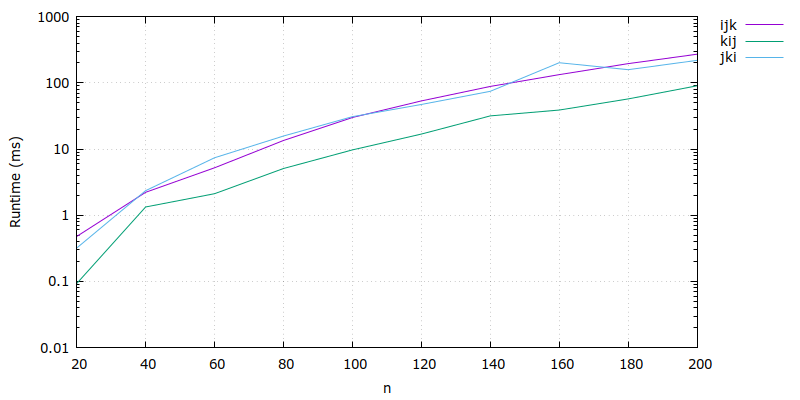
\includegraphics[width=\linewidth]{img/matmul.png}
    \caption{Benchmarking the different matrix multiplication
      implementations.  The $x$ axis shows the edge size of the
      matrices, while the logarithmic $y$ axis shows the runtime in
      milliseconds.  Note that the $kij$ loop ordering, which our
      analysis determined as optimal, is indeed about a factor of two
      faster than the other implementations.  Somewhat surprisingly,
      $iji$ (the original program) and $jki$ are about equally fast.
      This is possibly because the values of \texttt{n} used here are
      not as large as we assumed in our analysis.}
  \label{fig:matmul-graph}
\end{figure}

Our analysis shows that \cref{lst:matmul-kij.c} is the most
cache-efficient implementation.  Indeed, benchmarking these on a real
machine produces \cref{fig:matmul-graph}.  Note that all we did was
permute the loop ordering.  While obtaining true peak performance
typically requires more complicated program transformations than this,
we can often get quite far simply by carefully considering the order
in which we traverse our data.

%%% Local Variables:
%%% mode: latex
%%% TeX-master: "notes"
%%% End:
